\documentclass[journal,twoside,web]{ieeecolor}
\usepackage{generic}
\usepackage{cite}
\usepackage{amsmath,amssymb,amsfonts}
\usepackage{algorithmic}
\usepackage{graphicx}
\usepackage{algorithm,algorithmic}
\usepackage{hyperref}
\hypersetup{hidelinks=true}
\usepackage{textcomp}
% added packages
\usepackage{subcaption}
\graphicspath{{Fig/}}
\usepackage{booktabs}
\usepackage[flushleft]{threeparttable}
\usepackage{placeins}
%\usepackage{natbib}




\def\BibTeX{{\rm B\kern-.05em{\sc i\kern-.025em b}\kern-.08em
    T\kern-.1667em\lower.7ex\hbox{E}\kern-.125emX}}
\markboth{\hskip25pc IEEE TRANSACTIONS AND JOURNALS TEMPLATE}
{Author \MakeLowercase{\textit{et al.}}: Title}

\begin{document}
\title{DruGNNosis-MoA: Elucidating Drug Mechanisms as Etiological or Palliative With Graph Neural Networks Employing a Large Language Model}
\author{
%Brettler Liad, 
%Berman Eden,
%Jagodnik Kathleen M.,
%and 
%Bartal Alon
\thanks{
%All authors are with the The School of Business Administration, Bar-Ilan University, Ramat-Gan, 5290002, Israel (e-mail: alon.bartal@biu.ac.il).}
}
}
\maketitle

%Full names of authors are preferred in 

%the author field, but are not required.

%Put a space between authors' initials.

%The abstract must be between 150--250 words. 

% three or four different keywords or phrase

\begin{abstract}
Understanding the complex mechanisms of drugs' therapeutic effects is essential for advancing precision medicine and optimizing treatment strategies. 
However, systematically distinguishing between drugs that address root causes (etiological mechanisms) and those that alleviate symptoms (palliative mechanisms) using modern Artificial Intelligence (AI)-based strategies remains underexplored.
We present a novel computational framework for classifying drug Mechanisms of Action (MoA) as etiological or palliative, comparing three approaches: 
(i) Fine-tuning Science Bidirectional Encoder Representations from Transformers (SciBERT) with drug descriptions; 
(ii) Training various Graph Neural Networks (GNNs) on a constructed heterogeneous network of drugs, genes, and diseases; and 
(iii) Developing DruGNNosis-MoA, which integrates GNN with our fine-tuned SciBERT embeddings as node features. 
DruGNNosis-MoA excelled (F1-score 0.94) in identifying drug MoA. 
DruGNNosis-MoA characterizes drug mechanisms for subsequent pharmacological studies, thereby advancing precision medicine and therapeutic development.
\end{abstract}

\begin{IEEEkeywords}
%alphabetical order, separated by commas.
Etiological drugs;
Graph Neural Network (GNN);
Large Language Model (LLM);
Palliative drugs
\end{IEEEkeywords}

\section{Introduction}
\label{sec:intro}

\IEEEPARstart{M}{odern} medicine uses pharmaceutical interventions to combat diseases, alleviate symptoms, and support recovery through non-invasive treatment \cite{ravikumar2018improving,yu2020exploring}.
However, developing a new drug in the pharmaceutical industry is often prolonged, resource-intensive, and prone to frequent failures \cite{hammel2019new,xue2018review}.
Indeed, a considerable number of drug development initiatives fail to secure approval for public use, with critical issues frequently emerging at later stages of the drug discovery process \cite{hammel2019new}.
Preventing adverse reactions, balancing efficacy and toxicity, enhancing drugs, and addressing legal and financial factors add complexity to drug approval \cite{ravikumar2018improving}.

% Description of etiological and palliative drug mechanisms
Drugs can either directly target the underlying disease cause, or focus on alleviating a disease's symptoms \cite{yildirim2007drug,lindpaintner2002impact}.
Improving the drug design process can be informed by expanding our comprehension of these two fundamental drug mechanisms: 
(i) etiological -- targeting the root causes or contributing factors of a disease, and 
(ii) palliative -- alleviating symptoms by targeting proteins not directly implicated in the primary cause but involved in counteracting the disease's effects \cite{yildirim2007drug,lindpaintner2002impact}.
This distinction in drug mechanisms could guide the development of precise treatment strategies, minimizing side effects, optimizing resource allocation, and facilitating evidence-based healthcare decisions tailored to individual patients \cite{vogt2014molecularly}.

We note the distinction between the broad concept of drugs with palliative mechanisms (used to treat the general population, and the focus of the current project) and the narrower concept of drugs specifically used for end-of-life care, termed `palliative care', which typically employs opioids, anticholinergics, antipsychotics, and benzodiazepines for symptom relief during terminal illness \cite{jansen2018safety}.

Prior work \cite{yildirim2007drug,lindpaintner2002impact} suggested a connection between network distance and drug mechanism, motivating us to validate and extend these findings using more complex and advanced computational methods. 
We aim to explore whether network distance alone is sufficient to differentiate drug mechanisms of action, or if integrating multiple data sources (e.g., protein interactions, drug descriptions, disease associations) yields better predictions.

Yildirim et al. \cite{yildirim2007drug} proposed that in their network, distances greater than 1, which mirrored results from a randomized network, could be indicative of palliative drugs, while distances of 0 and 1, showing statistical significance, might represent etiological drugs.
Their findings suggest a prevalence of palliative drugs, with a smaller proportion of etiological ones.
They also speculated \cite{yildirim2007drug} that future developments might lead to a rise in the number of etiological drugs.
Our research validates this prediction.

More recently, \cite{guney2016network} analyzed large-scale datasets via network analysis to develop a drug-disease proximity measure to quantitatively assess the distances between drug targets and diseases, and categorize drugs as palliative or `effective' (comparable to our terminology of `etiological'). 
They concluded that their metric provides an unbiased measure of the therapeutic effects of drugs that permits the differentiation of `causative' (`effective') treatments from palliative ones. 
The authors reported that their network-based framework improves upon existing drug repurposing approaches, including similarity-based methods. 
As in our work presented here, \cite{guney2016network} assessed the Anatomic Therapeutic Chemical (ATC) classifications of proximal and distant drug-disease pairs and presented trends identified in these analyses.

% The difficulty in classifying drugs as etiological and palliative.
Distinguishing between etiological and palliative mechanisms of action (MoAs) involves challenges due to the complex nature of disease processes, potential overlap between targeting root causes and symptom relief, dual mechanisms exhibited by some drugs, limited treatment options for specific conditions, patient variability, the rarity of many diseases and conditions, and the interdisciplinary nature of healthcare \cite{yu2020exploring}.
The comprehensive classification of drugs based on MoAs is an under-studied aspect of drug research, motivating this study.

% Drug repurposing potential
The discovery of new drugs can also arise from drug repurposing \cite{parvathaneni2019drug}.
This involves identifying shared mechanistic characteristics among approved drugs, spanning related and additional Anatomical Therapeutic Chemical (ATC) classes \cite{xue2018review}.
Within the ATC classification system, active substances are grouped based on specific target organs or systems, as well as therapeutic, pharmacological, and chemical characteristics.
Leveraging the ATC classification facilitates the identification and exploration of potential drug treatments for new or under-studied diseases \cite{yang2017literature}.
For instance, \cite{olson2017predicting} utilized the ATC system to identify novel drug treatments for unstudied diseases.

% Prior work, introducing Lindpaintner and Yildirim
The systematic examination of etiological vs. palliative drug MoAs has received limited attention \cite{yildirim2007drug,lindpaintner2002impact,guney2016network}.
For instance, \cite{lindpaintner2002impact} provided examples to delineate this distinction, while \cite{yildirim2007drug} constructed networks that assessed drugs' proximity to diseases via protein interactions, and revealed an enrichment of palliative drugs.
Additionally, \cite{yildirim2007drug} proposed using the shortest distance between drug-target proteins and disease-gene product proteins as an indicator to classify drugs based on the molecular steps between a drug target and its associated disease cause.
Their finding suggests that short network distances between proteins indicate etiological mechanisms, while long distances suggest palliative mechanisms \cite{yildirim2007drug}. 
More recently, network analysis was used for drug screening \cite{guney2016network} that employs a drug-disease proximity measure quantifying relationships among drug targets and diseases, and assessing to what degree each drug is palliative vs. `effective'. 

% Other studies on different drug mechanism classification (literature review)
Numerous studies \cite{thafar2020dtigems+, sachdev2019comprehensive,vogt2014molecularly} of drug research and development have overlooked the crucial distinction between etiological and palliative mechanisms, neglecting the utilization of extensive datasets and contemporary analytical methods, such as Machine Learning (ML).
Other studies often focus on predicting drug-target interactions, repurposing \cite{fahimian2020repcool}, or drug mechanisms, lacking systematic classification \cite{vogt2014molecularly}.

% The opportunity available today to study these mechanisms using ML
Recent technological advances including the use of large-scale experimental validation of protein interactions, identification of disease-associated genes, and ML models, can aid in the field of drug discovery.
For example, a Graph Neural Network (GNN) is an ML model that captures the inherent qualities of a graph by transferring information between its nodes \cite{zhou2020graph}.
GNNs are effective for capturing complex patterns and dependencies in relational data.
Additionally, GNNs have been reported as highly effective in various graph analysis tasks, including node classification, link prediction, and graph clustering \cite{bongini2021molecular,jiang2021could,zhou2020graph}.
Leveraging the network's inherent structure, GNNs hold significant promise for revealing latent patterns and connections involving drug MoAs, facilitating the classification of drugs as having etiological or palliative MoA.

% Presenting three classification models
Drug classification based on etiological vs. palliative mechanisms of action has not been systematically researched using the most current available computational strategies.
To our knowledge, there has not yet been a model developed that categorizes drugs as having etiological or palliative mechanisms that employs GNNs or Large Language Models (LLMs).

Aiming to differentiate drugs with etiological vs. palliative mechanisms, we leveraged three extensive biomedical datasets, performing a comprehensive investigation of 2,018 U.S. FDA-approved drugs.
We developed three classification approaches:
(i) Fine-tuned a Science-BERT (SciBERT) model -- a Large Language Model (LLM) that was pre-trained \cite{beltagy2019scibert} on drug descriptions from DrugBank \cite{wishart2018drugbank,knox2024drugbank};
(ii) Trained various GNN models \cite{huang2020combining}; and
(iii) Trained a GNN model with node features extracted from drug descriptions processed by our fine-tuned SciBERT model, resulting in numerical embeddings.

% Goal and motivation
Our study innovates by employing advanced ML techniques to analyze extensive and diverse biomedical datasets for the elucidation of etiological and palliative drug mechanisms.
The systematic exploration of these mechanisms not only promises a paradigm shift in understanding drug actions but also holds the potential to reshape the landscape of early-stage drug discovery, refine personalized treatment selections, and optimize drug repurposing strategies.

%=========================================================
\section{Data}
\label{sec:materials}
%=========================================================
\subsection{Drug-Target Data}
\label{sec:DrugBank_data}
%-------------------------------------------------------
Using drug and gene target information from DrugBank (Version 5.1.10) \cite{wishart2018drugbank}, we recorded FDA-approved drugs targeting human genes, excluding those affecting retroviral genes. This process resulted in 2,018 drugs connected to 2,232 gene targets.
Drugs are represented by chemical IDs, and genes are represented by GenBank \cite{benson2012genbank} protein IDs and names.

%-------------------------------------------------------
\subsection{Protein–Protein Interaction (PPI) Data}
\label{sec:PPI_data}
%-------------------------------------------------------
We gathered experimentally validated PPIs in humans from the `Non-redundant' BioGRID database (Version 4.4.217) \cite{oughtred2021biogrid}.
We regard each interaction between protein \textit{A} and protein \textit{B} as bidirectional.
Identical interactions captured using a different experimental system or publication source were eliminated.
Proteins are represented by their official interactor gene symbols (i.e., gene names).
Hereafter, the proteins associated with genes are termed genes.
To ensure dataset coherence, we included only human genes, excluding PPIs associated with retroviruses.
The final dataset comprises 781,272 gene-gene interactions involving 19,893 genes within the human genome.

\subsection{Disease-Gene Data}
\label{sec:OMIM_data}
Information on the relationships between genotype and disease phenotype in humans was gathered from the Online Mendelian Inheritance in Man (OMIM) Morbid Map dataset (downloaded May 1, 2023) \cite{amberger2015omim}.
The dataset comprises OMIM's Synopsis of the Human Gene Map, encompassing 8,156 diseases and 16,358 disease-associated genes.
Diseases are represented by their phenotype name, while genes are represented by gene symbols.

%======================================================================================
\section{Methods
}\label{sec:methods}
%======================================================================================

\subsection{Drug Mechanism Labeling}
\label{sec:annotation}
%---------------------------------------------------------------------------------
Analyzing drug therapeutic mechanism information in DrugBank, we focused on the Identification and Pharmacology fields, including the Mechanism of Action subfield of the latter field, and manually classified each drug as having etiological (Class 1), palliative (Class 0), or both mechanisms. 
Each drug was annotated (Supplementary Table S1) by two independent annotators having bioinformatics training. 
In the case of conflicting labels, the discrepancy was discussed to achieve agreement on the final annotation.
This manual evaluation yielded an annotated dataset that delineates the mechanism of each drug.
For example, addressing vitamin deficiency, interventions such as replacement therapy or induced secretion of the deficient vitamin were classified as etiological, while drugs for alleviating the symptoms of the deficiency were labeled as palliative.
Our labeling approach aligns with the ATC classification framework, which groups drugs based on their primary therapeutic purpose. For example, drugs categorized under anti-infectives for systemic use (e.g., antibiotics) are generally etiological, targeting the cause of infections by acting on bacteria or viruses. In contrast, drugs classified under nervous system therapies (e.g., analgesics and anxiolytics) are typically palliative, focusing on relieving symptoms such as pain or anxiety without addressing the underlying disease causes.
We provide a list of publications that support our strategy for classifying drugs as having etiological or palliative mechanism (Supplementary Table S3) on the project’s GitHub repository.

\subsection{Fine-tuning SciBERT}
\label{sec:SciBERT}
We fine-tuned the SciBERT language model \cite{beltagy2019scibert} for classifying drugs as having etiological or palliative mechanism using drug descriptions from DrugBank and drug labels.
The Train data included text from the Pharmacodynamics and Mechanism of Action sections in DrugBank, with explicit indications of etiological or palliative mechanisms manually omitted to ensure that the model learned from a general context. 
The dataset was split into 90-10\% Train-Test sets, with the Train set further divided into a 10\% Validation set. 
We employed 10-fold cross-validation (CV) for fine-tuning SciBERT and assessed its performance using the F1-score.
%The best model, selected during CV, was then evaluated on the Test set.

\subsection{Network Modeling}
\label{sec:networks}

To reveal the complex relationships among diverse biological and pharmaceutical elements, we constructed four networks using the NetworkX Python package \cite{SciPyProceedings_11}.

%---------------------------------------------------------------------------------
\subsubsection{Network Construction}
\label{sec:network_construction_1}
%---------------------------------------------------------------------------------
\textbf{Drug-Target Network.}
Associates drugs and their target genes utilizing DrugBank data.
Designed as a bipartite graph, nodes correspond to drugs or target genes.
The network's links signify instances where a drug targets a specific protein translated from its associated gene.

\noindent\textbf{Protein-Protein Interaction (PPI) Network.}
Associates human proteins within a biological system based on BioGRID data.
Proteins are gene nodes, and two proteins are linked if a genetic interaction is reported.

\noindent\textbf{Disease-Gene Network.}
Associates diseases with their associated genes within OMIM Morbid Map.
Designed as a bipartite graph, nodes signify genes or diseases, and network links denote known associations between a gene and a disease.

\noindent\textbf{Heterogeneous Network.}
Using the Drug-Target, PPI, and Disease-Gene networks, we constructed a heterogeneous network.
Disease nodes connect genes associated with specific diseases, allowing DruGNNosis-MoA to identify drug-disease relationships based on shared gene associations.
This structure provides two insights: (i) Determining whether a drug mechanism is etiological or palliative based on gene connections; and (ii) Identifying patterns in drug use across diseases, which can suggest repurposing opportunities.
For example, in colorectal cancer, drugs targeting genes like KRAS (associated with cancer progression) are classified as etiological, while palliative drugs, such as analgesics, address symptoms like pain.
This approach helps researchers to identify drug repurposing opportunities, develop more balanced treatment strategies, and guide drug discovery by pinpointing unmet therapeutic needs.

To facilitate binary classification, drugs displaying a dual role of both etiological and palliative mechanisms were excluded.
We utilized the heterogeneous network for the development of GNN models.
Nodes of the heterogeneous network represent drugs, genes, and diseases.
Each drug node has a label attribute indicating either etiological or palliative mechanism.
Links (edges) of the heterogeneous network include: drug-gene (targeting), gene-gene (protein interaction), and disease-gene (association).
Next, we trained a GNN models using the PyTorch Geometric (PyG) library with our heterogeneous network \cite{Fey/Lenssen/2019}.

%-----------------------------------------------------------
\subsubsection{Graph Neural Network Model Development}
\label{sec:model}
%-----------------------------------------------------------
Given the strengths of GNNs in node classification, particularly in capturing complex relationships within graph structures, we trained four GNN classifiers:
SAGEConv  \cite{hamilton2017inductive}, 
GATConv \cite{velivckovic2017graph}, 
GATv2Conv  \cite{brody2021attentive}, and 
GraphConv  \cite{kipf2016semi}
on our heterogeneous network.
These models were chosen for their proven effectiveness in biological and biomedical applications, where they excel at learning from  heterogeneous data structures. 
This capability aligns well with the data characteristics used in developing our DruGNNosis-MoA model.

\textbf{Baseline GNNs.}
Given the heterogeneous network, we assign the EigenVector decomposition for each node \cite{huang2020combining}, capturing informative node features.
We standardized these EigenVectors using Z-score normalization for subsequent analysis that include the following GNNs as baseline models:
SAGEConv, GATConv, GATv2Conv, and GraphConv, as well as SciBERT, and our fine-tuned SciBERT LLMs.

\textbf{DruGNNosis-MoA.}
Given the heterogeneous network, we integrated textual features (embeddings) for each node.
To generate textual node features, we applied our fine-tuned SciBERT model on drug descriptions from DrugBank; gene symbols from PPI data; and disease names from OMIM.
We then reduced the dimensionality of text embeddings from the fine-tuned SciBERT model to size 128 using Principal Component Analysis (PCA), thus enhancing the foundational feature input for the DruGNNosis-MoA model.
This reduction focuses the model on the most relevant aspects of the data.
Lastly, a GNN was applied to the graph to classify nodes.


%-----------------------------------------------------------
\subsubsection{Graph Neural Network Training}
\label{sec:Train}
%-----------------------------------------------------------
We divided drug nodes into Train (90\%) and Test (10\%) sets, implementing a 10-fold cross-validation (CV) on the Train set, reserving 10\% of the Train set as a Validation set in each fold.
Both the partitioning and CV were conducted in a stratified manner, ensuring a balanced and proportional distribution of each label class and mitigating the risk of biased model training.
We applied a transductive node classification approach, enabling all sets to access the complete graph structure.
However, they were limited to knowing only the labels of the nodes within their respective subsets.
After the CV process, we applied our DruGNNosis-MoA model to the independent Test set.
This final evaluation provided an unbiased assessment of the model’s generalizability, with no overlap between the Train and Test sets in terms of labeled data.


%-----------------------------------------------------------
\subsection{Model Evaluation}
%-----------------------------------------------------------
To ensure a fair comparison among the fine-tuned SciBERT, the Baseline GNNs, and the DruGNNosis-MoA models in terms of MoA classification, we used the same 10-fold CV process to evaluate their performances.
The average cross-validation F1-score, and area under the curve (AUC) were reported for each model.
To determine the best-performing model, we compared the averages F1-scores and ROC-AUC scores across the models.
Finally, the performance of the selected best model was evaluated on the Test set.

Fig. \ref{fig:FlowChart} summarizes the methods employed in this study.


\begin{figure*}
    \centering
    \includegraphics[scale=0.7, trim={4cm 2.5cm 2cm 2cm}, clip]{Figures/FlowChart3.pdf}
    \caption{Flowchart of methods employed in this study to build our DruGNNosis-MoA model.
            Illustration of the sequential steps employed to classify drugs as having either etiological or palliative mechanism.
            In Step 1, we acquired and processed our selected datasets, which comprise information on drugs, genes, and diseases.
            In Step 2, we constructed three distinct networks for Drug-Target, Gene-Gene, and Disease-Gene interactions.
            In Step 3, these networks were then integrated to form a comprehensive Heterogeneous network, encompassing a diverse range of node and link (edge) types.
            Following the network integration, in Step 4, we calculated feature embedding on each node type individually utilizing our fine-tuned SciBERT model \cite{beltagy2019scibert}.
            Finally, In Step 5, we streamlined the network embeddings through our Graph Neural Network (GNN) to carry out the classification task, distinguishing each drug node as either etiological or palliative.
    }
    \label{fig:FlowChart}
\end{figure*}


%-----------------------------------------------------------
\section{Results}
\label{sec:res}
%-----------------------------------------------------------
We began by manually labeling drugs as etiological and palliative.
Using the labeled set of drugs, we fine-tuned the SciBERT model to classify drugs as etiological or palliative.
Next, we constructed biological networks and trained GNNs with different configurations.
Finally, we compared the performances of the baseline models vs. our DruGNNosis-MoA model.
%We review the results of these analyses in this section.

%-----------------------------------------------------------
\subsection{Drug Mechanism Labeling}
%-----------------------------------------------------------
A residual drug subset (3.816\%, 77) exhibited a dual role of both etiological and palliative mechanisms based on the diseases they address.
This subset was discarded to implement binary classification.
For example, methotrexate acts as a drug with etiological mechanism in cancer treatment by inhibiting cell division, and acts as a drug with palliative mechanism in arthritis treatment by reducing inflammation.
The remaining drugs present a nearly equal distribution of either etiological (47.423\%, 957) or palliative (48.761\%, 984) mechanisms (Supplementary Fig. S1). %\ref{fig:EvsP}).
This differs from \cite{yildirim2007drug}, which reported a prevalence of palliative drugs.
Possible reasons for this difference include the potential changes in drug design trends over 16 years, and the undisclosed classification method \cite{yildirim2007drug}.


Drugs affiliated to multiple Anatomical Therapeutic Chemical (ATC) classes suggest the possibility of repurposing by utilizing them in different therapeutic categories.
We analyzed how drug mechanisms are distributed across ATC classes (Supplementary Fig. S2)%\ref{fig:EPvsATC})
, inspired by the work of \cite{yildirim2007drug}, who did not directly analyze this distribution \cite[Fig. 2]{yildirim2007drug}.
Our analysis revealed distinct distributions within each class.
In the `Nervous System' class, most drugs are palliative (88.484\%, 292), addressing symptoms like pain and psychiatric disorders, but not their underlying causes.
In contrast, drugs in the `Antiinfectives for Systemic Use' class mainly have etiological mechanisms (90.476\%, 57), targeting the root cause of infections such as bacteria and viruses.
Dual-mechanism drugs, addressing both causes and symptoms, make up a small percentage (1.587\% to 7.746\%) across all classes.
This indicates diverse drug roles in different therapeutic areas.

\textbf{Analyzing drug-disease distances.}
The methodology of \cite{yildirim2007drug} lacked specifics on selecting drug-disease pairs.
To address this gap, we examined three distinct strategies for calculating drug-disease distances (see Supplementary Fig. S3), yielding a more nuanced view of drug classification.
The All vs. All (Comprehensive) Method examines all possible paths between each drug and disease pair.
These results, as depicted in Fig. S3a%\ref{fig:yildirim1}
, exhibit the most resemblance to \cite{yildirim2007drug}'s findings that are presented in \cite[Fig. 6a]{yildirim2007drug}.
When excluding instances of drug duplicates from the same distance, using the All vs. All (Unique) Method depicted in Fig. S3b, %\ref{fig:yildirim2}, 
the distribution of drug mechanisms is similar at most distance values.
This indicates that almost every drug has a corresponding disease at each distance.
We believe that the Unique Minimum Shortest Distance Method, shown in Fig. S3c, %\ref{fig:yildirim3}, 
offers the most insightful analysis.
This method reveals a significant concentration of connections at distances 0 and 1, aligning with \cite{yildirim2007drug}'s observations of statistical significance.
However, contrary to \cite{yildirim2007drug}'s suggestion, this method demonstrates a combination of drugs with etiological and palliative mechanisms within each distance.
For example, at distance 1, there are 218 drugs with etiological mechanisms and 136 drugs with palliative mechanisms.
This challenges the notion that distances greater than $1$ predominantly represent drugs with palliative mechanisms. Consistent with this finding that drugs with etiological vs. palliative mechanisms cannot be neatly assessed for mechanism simply by inspecting the network distance, Wang et al. \cite{wang2012relationship} reported that their groups of etiological and palliative drugs each had a median distance of 4; however, they noted that palliative drugs have a higher fraction of network distance 4 than etiological drugs.


%-----------------------------------------------------------
\subsection{Fine-tuning SciBERT}
%-----------------------------------------------------------
Using drug labeling in the previous section, we fine-tuned the SciBERT model to predict drug labels.
For text inputs into SciBERT, we sourced drug descriptions from DrugBank; gene symbols from BioGRID; and disease names from OMIM.
Following the guidelines of \cite{devlin-etal-2019-bert}, we utilized the Trainer class from Hugging Face \cite{wolf2019huggingface}, with the following parameters:
AdamW optimizer with a weight decay of  $2e^{-3}$.
AdamW differs from standard Adam by its unique approach to weight decay regularization; a learning rate of $2e^{-5}$; a batch size of 16; and a total of 3 training cycles.


SciBERT represented each text as a numeric vector (embeddings vector) of size 768.
Consequently, we obtained three unique matrices of $Entity \times 768$ dimensionality, where Entity (rows) indicate either drugs, genes or diseases; and columns indicate values of the embeddings vectors.
Then, we performed Principal Component Analysis (PCA) to reduce the dimensionality of each matrix to $Entity \times 128$.
The reduced embedding vector for each entity type was integrated into our heterogeneous network as a node (drug, gene, disease) feature.
This integration enhanced the learning capabilities of the GNN in developing more robust and representative node features.


%-----------------------------------------------------------
\subsection{Network Construction}
\label{sec:network_construction_2}
%-----------------------------------------------------------

An overview of the networks analyzed in this project is presented in Table \ref{tbl:networkFeatures}, and descriptions are provided below.

\textbf{Drug-Target Network}
comprises 2,018 drug nodes, 2,232 target-gene nodes, and 10,250 links (edges) connecting them.
It forms 129 connected components, with 75 consisting of standalone drug-target pairs.
We observe a small number of highly connected nodes (hubs) and numerous nodes with only a few connections \cite{barabasi2009scale}.
The Largest Connected Component (LCC) within the network includes 1,797 drug nodes, 2,027 target-gene nodes, and 9,916 links.
Notably, the most frequent degree in the LCC is 1, suggesting a prevalence of nodes with a single connection.
Higher degrees are less frequent, aligning with the hubs that determine the connectivity of the LCC.

\textbf{PPI Network}
comprises 19,893 gene nodes interconnected by 781,272 links, excluding 3,344 self-interactions.
This network has 4 components, with 3 of them consisting of isolated genes.
The most frequent degree is 1, indicating a prevalence of branched-off nodes with a single connection.

\begin{table}
\caption{Summary descriptions of the analyzed networks.
\label{tbl:networkFeatures}}%
\begin{threeparttable}
\begin{tabular*}{\columnwidth}{@{\extracolsep\fill}llll@{\extracolsep\fill}}
\toprule
Network & \# Nodes  & \# Links (Edges)\\
\midrule
Drug-Target               & 2,018 drugs    & 10,250\\
                          & 2,232 genes            \\
\midrule
PPI                       & 19,893 genes   & 781,272\\
\midrule
Disease-Gene              & 8,156 diseases & 27,692\\
                          & 16,358 genes           \\  
\midrule
Heterogeneous\tnote{*}    & 1,941 drugs   & 822,086\\
                          & 31,524 genes           \\
                          & 8,156 diseases         \\
\bottomrule
\end{tabular*}
\begin{tablenotes}
\item[*] The heterogeneous network's topological features were calculated while excluding drugs labeled as having `both' etiological and palliative mechanisms.
\end{tablenotes}
\end{threeparttable}
\end{table}




\textbf{Disease-Gene Network}
comprises 8,156 disease nodes, 16,358 associated-gene nodes, and 27,692 links (edges) connecting them.
This network is organized into 5,430 connected components, with 1,065 being standalone disease-gene pairs.
Each component features a unique set of diseases and genes that are closely interconnected.
Within this network, the LCC consists of 265 disease nodes, 379 associated-gene nodes, and 1,493 links (edges).
The most frequent degree in the LCC is 2, indicating that the majority of diseases or genes in this component are connected to two other genes or diseases.


\textbf{Heterogeneous Network}
comprised of 1,941 drug nodes (excluding those with both etiological and palliative mechanisms), 31,524 gene nodes, and 8,156 disease nodes.
The link types include 9,778 drug-gene links, 784,616 gene-gene links, and 27,692 disease-gene links, for a total of 822,086 edges.

Topological network analyses revealed a significant occurrence of ``follow-on" drugs.
These are drugs that target proteins that have already been selected targets for previous drugs.
This trend reflects a prevailing strategy within the pharmaceutical industry to concentrate efforts on well-established target proteins, resulting in an accumulation of such drugs that target proteins already targeted by existing drugs \cite{aronson2020me}.
This strategy limits drug discovery to a narrow range of target proteins, restricting the exploration of novel targets

Fig. \ref{fig:heteroSubGraph} illustrates a sub-graph of our heterogeneous network exhibiting the occurrence of follow-on drugs linked to colorectal cancer (green) genes.
Within this sub-graph, there are a total of 48 genes (blue) associated with colorectal cancer, with some connections to other genes.
A smaller subset of these genes is targeted by drugs (orange), revealing a clustering effect of drugs focused on specific targets.
Notably, the majority of these drugs are categorized as having etiological mechanisms, aligning with our findings that most drugs designed to combat cancer primarily work by inhibiting cell division and hindering growth.
Our trained GNN models utilize this heterogeneous network for learning how to classify drugs as having either etiological or palliative mechanism.

We tested different GNN classifiers, trained both with and without textual features: models without textual features used Eigenvector features, while models with textual features, including our DruGNNosis-MoA model, incorporated embeddings from our fine-tuned SciBERT model.
In all models, drug nodes were labeled as either etiological or palliative.
For GNNs training information, see Supplementary Table S2. 


\begin{figure}
    \centering
    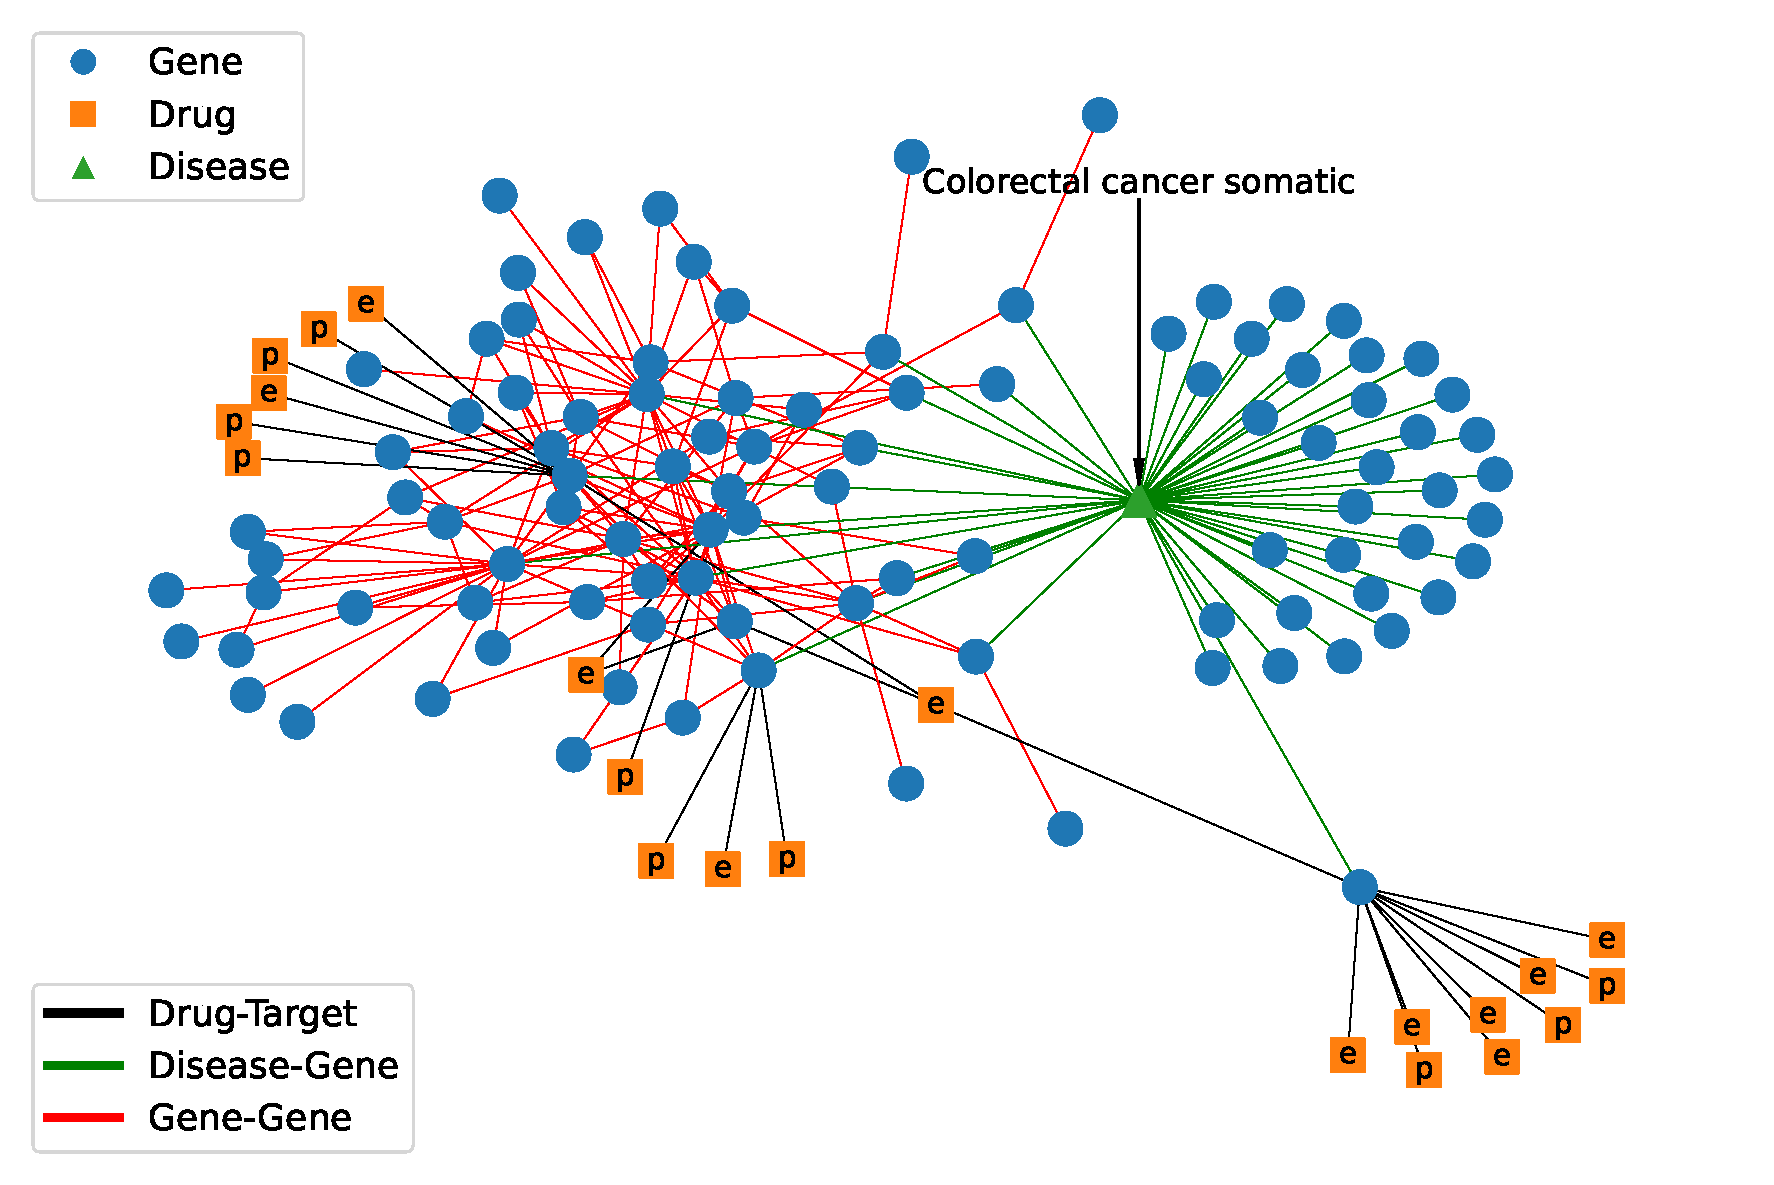
\includegraphics[width=\linewidth]{Figures/heterogeneous_networks.pdf}
    \caption{ \text{Example sub-graph of our heterogeneous network}. The disease colorectal cancer (green triangle) is connected directly and indirectly to numerous genes (blue dots).
    For visualization purposes, we selected all directly linked genes, and some indirectly linked genes, to sum to 50 in total.
    Some of these genes are targeted by drugs (orange squares). Each drug is labeled as having etiological (`e') or palliative (`p') mechanism.
    ``Follow-on" drugs, which are drugs targeting the same gene as other drugs, can be seen.
    This network shows the existence of many potential gene targets for colorectal cancer, yet only a few have been selected for drug treatment, to date. Additionally, this sub-graph reveals a dominance of etiological drugs, correlating with our findings of the `L’ ATC class.}
    \label{fig:heteroSubGraph}
\end{figure}


%-----------------------------------------------------------
\subsection{DruGNNosis-MoA Training}
%-----------------------------------------------------------
Our DruGNNosis-MoA model was trained over 30 epochs using two SageConv layers, a ReLU activation function, and the Adam optimizer with a learning rate of \(6 \times 10^{-4}\).
We applied a sigmoid function to the output and implemented gradient clipping with a threshold of 0.5 to ensure stable training.
To prevent overfitting, we incorporated an additional dropout strategy in our DruGNNosis-MoA model after the first layer, set at a probability of 0.3.
Dropout randomly deactivates a portion of nodes during training, reducing overfitting by preventing complex co-adaptations on Train data.


During the training of all GNNs, the graph structure was accessible to the models across all sets, following the transductive learning \cite{mishra2020node}, meaning that only structural information (i.e., node connectivity reflected in known biomedical datasets) was available to the model, ensuring no leakage of ground truth labels. 
Additionally, only node labels of the Train set were provided during training, ensuring that no label information from the Test nodes was present during model training.

%-----------------------------------------------------------
\subsection{Model Evaluation}
%-----------------------------------------------------------
For model comparison, we employed a 10-fold CV process on the Train set to tune hyperparameters and select the best-performing model. 
This process ensured that the model was trained and validated on multiple partitions, mitigating any overfitting to a particular subset. 
Importantly, the Test set remained completely unseen to our model during the CV process and was only used for final model performance estimation. 
For each fold, we computed the F1-scores and ROC-AUC score (Area Under the Curve). 
We then calculated the average score for each metric (Table \ref{tbl:cv_scores}).

%\begin{table}
%\caption{Cross-validation metric scores of different models.
%\label{tbl:cv_scores}}%
%\begin{tabular*}{\columnwidth}{@{\extracolsep\fill}lll@{\extracolsep\fill}}
%\toprule
%Model & Metrics & Average \\
%\midrule
%Baseline GNN & Accuracy    & 0.699   \\
%             & F1-score         & 0.664   \\
%             & Precision         & 0.715   \\
%             & Recall            & 0.622    \\
%             & ROC-AUC     & 0.787   \\
%\midrule
%SciBERT & Accuracy    & 0.820    \\
%            & F1-score         & 0.810   \\
%            & Precision         & 0.850   \\
%            & Recall            & 0.780   \\
%            & ROC-AUC     & 0.910   \\
%\midrule
%Fine-Tuned SciBERT & Accuracy    & 0.906   \\
%                   & F1-score         & 0.906   \\
%                   & Precision         & 0.895   \\
%                   & Recall            & 0.918   \\
%                   & ROC-AUC     & 0.961   \\
%\midrule
%DruGNNosis-MoA & Accuracy    & 0.938    \\
%            & F1-score         & 0.935   \\
%            & Precision         & 0.931   \\
%            & Recall            & 0.941   \\
%            & ROC-AUC     & 0.977   \\
%\bottomrule
%\end{tabular*}
%\begin{tablenotes}%
%\end{tablenotes}
%\end{table}


\begin{table}
\caption{Cross-validation F1-score averages of models.}
\label{tbl:cv_scores}%
\begin{tabular*}{\columnwidth}{@{\extracolsep\fill}ll@{\extracolsep\fill}}
\toprule
Model & F1-score \\
\midrule
DruGNNosis-MoA (SAGEConv + Fine-Tuned SciBERT) & 0.935 \\
SAGEConv & 0.664 \\
Fine-Tuned SciBERT & 0.906 \\
SciBERT & 0.815 \\
GATConv + Fine-tuned SciBERT & 0.791 \\
GATConv & 0.665 \\
GATv2Conv + Fine-tuned SciBERT & 0.833 \\
GATv2Conv & 0.682 \\
GraphConv + Fine-tuned SciBERT & 0.829 \\
GraphConv & 0.711 \\
\bottomrule
\end{tabular*}
\end{table}



DruGNNosis-MoA outperformed all other models.
The non-fine-tuned SciBERT achieved an F1-score of 0.815, versus 0.906 for the fine-tuned model, showing the impact of domain-specific fine-tuning. 
DruGNNosis-MoA further raised the F1-score to 0.935 (Table \ref{tbl:cv_scores}), highlighting the added value of graph-based learning for improved accuracy and generalizability.

We then closely examined the performance trends of the two top models, fine-tuned SciBERT and DruGNNosis-MoA (Fig. S4). % \ref{fig:fscore1b})
The DruGNNosis-MoA model shows higher F1-scores in every fold when compared with the fine-tuned SciBERT model.
This pattern suggests a trend where DruGNNosis-MoA outperforms the fine-tuned SciBERT in the task of classifying drugs as having etiological or palliative mechanisms (Fig. S4). %\ref{fig:fscore1b}).

After observing that the DruGNNosis-MoA model demonstrated superior performance for F1-score, we assessed its efficacy compared with other tested models via the ROC-AUC curve that presents an average AUC score (Fig. \ref{fig:roc_auc1}).



The ROC-AUC curve, as shown in Fig. \ref{fig:roc_auc1}, 
demonstrates the DruGNNosis-MoA model's consistently superior performance in classifying drugs.
It achieves an impressive average Area Under the Curve (AUC) of 0.98.
These results indicate a difference in performance between the DruGNNosis-MoA model and other evaluated models, with implications for their respective efficacy in drug classification tasks.

Overall, we observe that our DruGNNosis-MoA model outperformed all other models (Table \ref{tbl:cv_scores}).
In the evaluation of the DruGNNosis-MoA model, the highest standard deviation (S.D.) observed was 0.029 in the precision metric, while the lowest S.D., 0.001, was found in the ROC-AUC metric.
Notably, this ROC-AUC S.D. is the smallest across all matrices and models.

Finally, we applied the DruGNNosis-MoA model to our Test set,
resulting in an F1-score of 0.94 and a ROC-AUC value of 0.97.
These results further reinforce the consistent superiority of the DruGNNosis-MoA model in drug classification performance on previously unseen data.


\begin{figure}
\centering
   \includegraphics[width=\linewidth]{Figures/avg_roc_scores2.png}
   \caption{
    Receiver Operating Characteristic (ROC) curve for baseline models and DruGNNosis-MoA in classifying drugs as having etiological or palliative mechanism. 
    The ROC curve illustrates model performance over 10-fold cross-validation.}
\label{fig:roc_auc1}
\end{figure}



%-----------------------------------------------------------
\subsubsection{Model Evaluation on Sparse Data}
\label{sec:sparse_data_evaluation}

Given the challenges associated with diseases and drugs that have few verified gene associations, we evaluated the performance of our DruGNNosis-MoA model under sparse data conditions.
This evaluation is critical for understanding the model's reliability in low-sample scenarios, particularly for rare diseases and sparsely annotated conditions.

DruGNNosis-MoA uses neighborhood aggregation to enrich sparse nodes by propagating information from well-connected neighbors.
Additionally, dropout during training prevents overfitting to dense nodes, enhancing generalization to sparse data.

We validated model performance on sparse data from our independent Test set, focusing on drugs with 1 to 10 gene associations, and evaluating classification accuracy (etiological vs. palliative) via F1-score against baseline models.

Fig. \ref{fig:class} shows (a) a visualization of classification results for the independent Test set, and (b) the F1-score performance of DruGNNosis-MoA, for drugs associated with 1 to 10 genes. 
Our results demonstrate that DruGNNosis-MoA performs consistently well, even for drugs with few associated genes, validating its reliability in low-sample scenarios.
We further analyzed the full dataset for gene associations per drug (Fig. \ref{fig:genes_per_drug}) and found that most drugs had few associations. 

The results show that DruGNNosis-MoA effectively handles sparse data, demonstrating its value for classifying drugs with limited gene-disease associations, including rare diseases.


\begin{figure}
\centering
   \includegraphics[width=\linewidth]{Figures/fig4.pdf}
   \caption{
            (a) Visualization of classification results on the independent Test set.
            (b) DruGNNosis-MoA performance (F1-score) broken down by the number of gene associations per drug, specifically for drugs with 1 to 10 gene associations.
            }
\label{fig:class}
\end{figure}



\begin{figure}
\centering
   \includegraphics[width=\linewidth]{Figures/fig5.pdf}
   \caption{
             Distribution of the number of gene associations per drug in the full analyzed dataset, highlighting the prevalence of low-association drugs.
            }
\label{fig:genes_per_drug}
\end{figure}


%--------------------------------
\section{Discussion and Conclusions}
%--------------------------------
Elucidating drug mechanisms as etiological or palliative is crucial for drug design and treatment selection. 
Understanding these mechanisms can guide the development of new drugs and the repurposing of existing ones. 
Our findings show a balance between etiological and palliative mechanisms among FDA-approved drugs.

Our work advances systematic drug mechanism classification by combining large language models (LLMs) and graph-based learning, extending beyond previous network-based analyses to improve predictions of drug mechanisms.
The distinction between etiological and palliative mechanisms prompts a consideration of whether a drug aims to address root causes or alleviate symptoms. 
This differentiation is vital for advancing medical treatments.

The combination of a GNN model and our fine-tuned SciBERT model in DruGNNosis-MoA outperformed all other models. 
This hybrid approach of DruGNNosis-MoA that integrates both fine-tuned SciBERT embeddings as node features and a GNN, offers a key advantage: the GNN captures topological relationships that are not accessible to the language model, improving generalization to scenarios involving complex or sparse data.

Our novel DruGNNosis-MoA model integrates diverse data, uncovering hidden relationships in drug-gene-disease interactions. 
This study is pioneering in using a language-network framework with machine learning to explore these mechanisms, offering insights beyond conventional distance-based methods.

The work of Yildirim et al. \cite{yildirim2007drug} anticipated a growth in the development of drugs with etiological mechanisms, a hypothesis we explored in this paper.
We found limitations in their approach \cite{yildirim2007drug} of relying solely on distances within the network for drug mechanism classification.
Our replication of the analyses of \cite{yildirim2007drug} did not reveal a significant correlation between drug mechanisms and network distance, as both mechanism types appeared at short and long distances. 
While short distances may sometimes reflect etiological mechanisms \cite{yildirim2007drug}, our findings show no consistent correlation between network distance and drug mechanisms, indicating that our DruGNNosis-MoA model is more reliable than network distance-based approaches for predicting drug MoAs.
This difference in results from prior studies may be due to our advanced computational approach to identifying drug MoA.

Examining individual ATC classes revealed that the balance of etiological and palliative mechanisms does not apply universally.
We also identified drugs with dual mechanisms, challenging the binary classification and highlighting the complexity of drug actions.

Our method's limitations include potential subjectivity in labeling drug mechanisms as etiological or palliative, based on DrugBank data.
Some drugs are associated with multiple disease conditions, complicating their classification. 
Future work should refine these labels and explore specific drug mechanisms in detail.

We acknowledge that labeling a drug as having an etiological mechanism of action does not imply a cure, as some data include diseases not officially approved for treatment, and many drugs with etiological mechanisms are only partially effective. 
Expanding features included in our model, such as chemical structures, could improve model performance.
Additionally, future studies should explore the integration of advanced GNN architectures to further improve the performance of DruGNNosis-MoA. 
Specifically, Fuzzy Logic-Enhanced GNNs \cite{yang2023fuzzy} show promise by incorporating uncertainty modeling into graph learning processes, which could be particularly beneficial for handling noisy or incomplete biomedical data.
Dynamic graph models could further improve predictive accuracy by capturing temporal changes in drug-disease relationships, such as evolving clinical knowledge or emerging drug repurposing opportunities.
Future employment of these advanced GNN techniques can enhance the generalizability and adaptability of DruGNNosis-MoA for more complex and evolving biomedical applications.
Finally, future research can explore experimental drug datasets to assess their applicability to drugs with unknown MoAs.


Our study offers avenues for further research, including exploring novel drug targets, analyzing therapeutic success rates by drug mechanism, and focusing on specific ATC classes for a deeper understanding of relationships within the network.
Our approach advances the systematic assessment of drug mechanisms using cutting-edge computational methods, enhancing precision and efficiency in drug development and repurposing.


%\section{Competing interests}
%The authors declare no competing interests.

%\section{Author contributions statement}
%L.B. contributed Investigation, Formal Analysis, Methodology, Software, Validation, Visualization, Writing – original draft, and Writing - review and editing. 
%E.B. contributed Investigation, Formal Analysis, Data curation, Validation, Visualization, Writing – original draft, and Writing - review and editing. 
%K.M.J. contributed Conceptualization, Data curation, Funding acquisition, Methodology, Project administration, Supervision, Validation, Visualization, Writing – original draft, and Writing – review and editing. 
%A.B. contributed Conceptualization, Formal analysis, Funding acquisition, Investigation, Methodology, Project administration, Resources, Software, Supervision, Visualization, Writing – original draft, and Writing – review and editing.

%\section{Acknowledgments} 
%This work is supported in part by funds from Bar-Ilan University's Data Science Institute (DSI). K.M.J. was funded by a Postdoctoral Fellowship from the Mortimer B. Zuckerman STEM Leadership Program.


%square brackets. 
%Multiple references are each numbered with separate brackets. 
%---------------------------------------------------------------------
\section*{Acknowledgment}
%---------------------------------------------------------------------


%---------------------------------------------------------------------
\bibliographystyle{IEEEtran} % or ieeetr, plain, etc.
\bibliography{References}
%---------------------------------------------------------------------

\end{document}
